%%%%%%%%%%%%%%%%%%%%%%%%%%%%%%%%%%%%%%%%%
% Memo
% LaTeX Template
% Version 1.0 (30/12/13)
%
% This template has been downloaded from:
% http://www.LaTeXTemplates.com
%
% Original author:
% Rob Oakes (http://www.oak-tree.us) with modifications by:
% Vel (vel@latextemplates.com)
%
% License:
% CC BY-NC-SA 3.0 (http://creativecommons.org/licenses/by-nc-sa/3.0/)
%
%%%%%%%%%%%%%%%%%%%%%%%%%%%%%%%%%%%%%%%%%

\documentclass[letterpaper,11pt]{texMemo} % Set the paper size (letterpaper, a4paper, etc) and font size (10pt, 11pt or 12pt)

\usepackage{parskip} % Adds spacing between paragraphs
\usepackage[colorlinks]{hyperref}
\usepackage{graphicx}
\usepackage{float}
\usepackage{hyperref}
\usepackage{listings}
\hypersetup{citecolor=DeepPink4}
\hypersetup{linkcolor=red}
\hypersetup{urlcolor=blue}
\usepackage{cleveref}
\setlength{\parindent}{15pt} % Indent paragraphs

%----------------------------------------------------------------------------------------
%	MEMO INFORMATION
%----------------------------------------------------------------------------------------

\memoto{Dr.Randy Hoover} % Recipient(s)

\memofrom{Benjamin LeBrun, Benjamin Garcia} % Sender(s)

\memosubject{Lab Assignment 6: TC1 and Ultrasonic Sensors} % Memo subject

\memodate{\today} % Date, set to \today for automatically printing todays date

% \logo{\includegraphics[width=0.1\textwidth]{logo.png}} % Institution logo at the top right of the memo, comment out this line for no logo

%----------------------------------------------------------------------------------------

\begin{document}

\maketitle % Print the memo header information

%----------------------------------------------------------------------------------------
%	MEMO CONTENT
%----------------------------------------------------------------------------------------

\section*{Introduction}
This lab tasked us with configuring the provided HC-SR04 ultrasonic range sensor using the ATMega328P's Timer/Counter1. We then had to provide a linear mapping from $[3cm,30cm]->[0,255]$ and control the robot's motor speed using this mapping. The sensor output and appropriate mapping was to then be displayed to the screen with every distance sample.

\section*{Equipment}
While the lab used the entire robot kit assembled together, the primary devices
we used were:

\begin{itemize}
    \item Acrylic vehicle body with screws, assembled
    \item Elegoo Uno (chip: Atmega328p)
    \item 4 DC motors with wheels, screws 
    \item L298 H bridge module dual channel
    \item 2 ICR18650 batteries with battery box
    \item Ribbon cables
    \item Host laptop with AVR-gcc 8-bit toolchain
    \item USB 2.0 A to B cable
    \item HC-SR04 ultrasonic range sensor
\end{itemize}

\subsection*{Configuration}
Our robot vehicle was assembled according to Elegoo's instructions which can be found
on Elegoo's website at \url{https://www.elegoo.com/download/}. For this lab, we are
using the V3.0 version of the robot kit.

The ultrasonic sensor, battery pack, and H bridge were connected to the marked locations on the Elegoo shield included in the kit. The wheel motors were connected two to a side with the H bridge in the lower portion of the robot.

While the motors require more power than the micro-controller can provide to operate, the ultrasonic sensor is capable of running off of the micro-controller's power. Both components are capable of running off of the kit-provided battery pack when it is switched on.

\begin{figure}[!ht]
\begin{center}
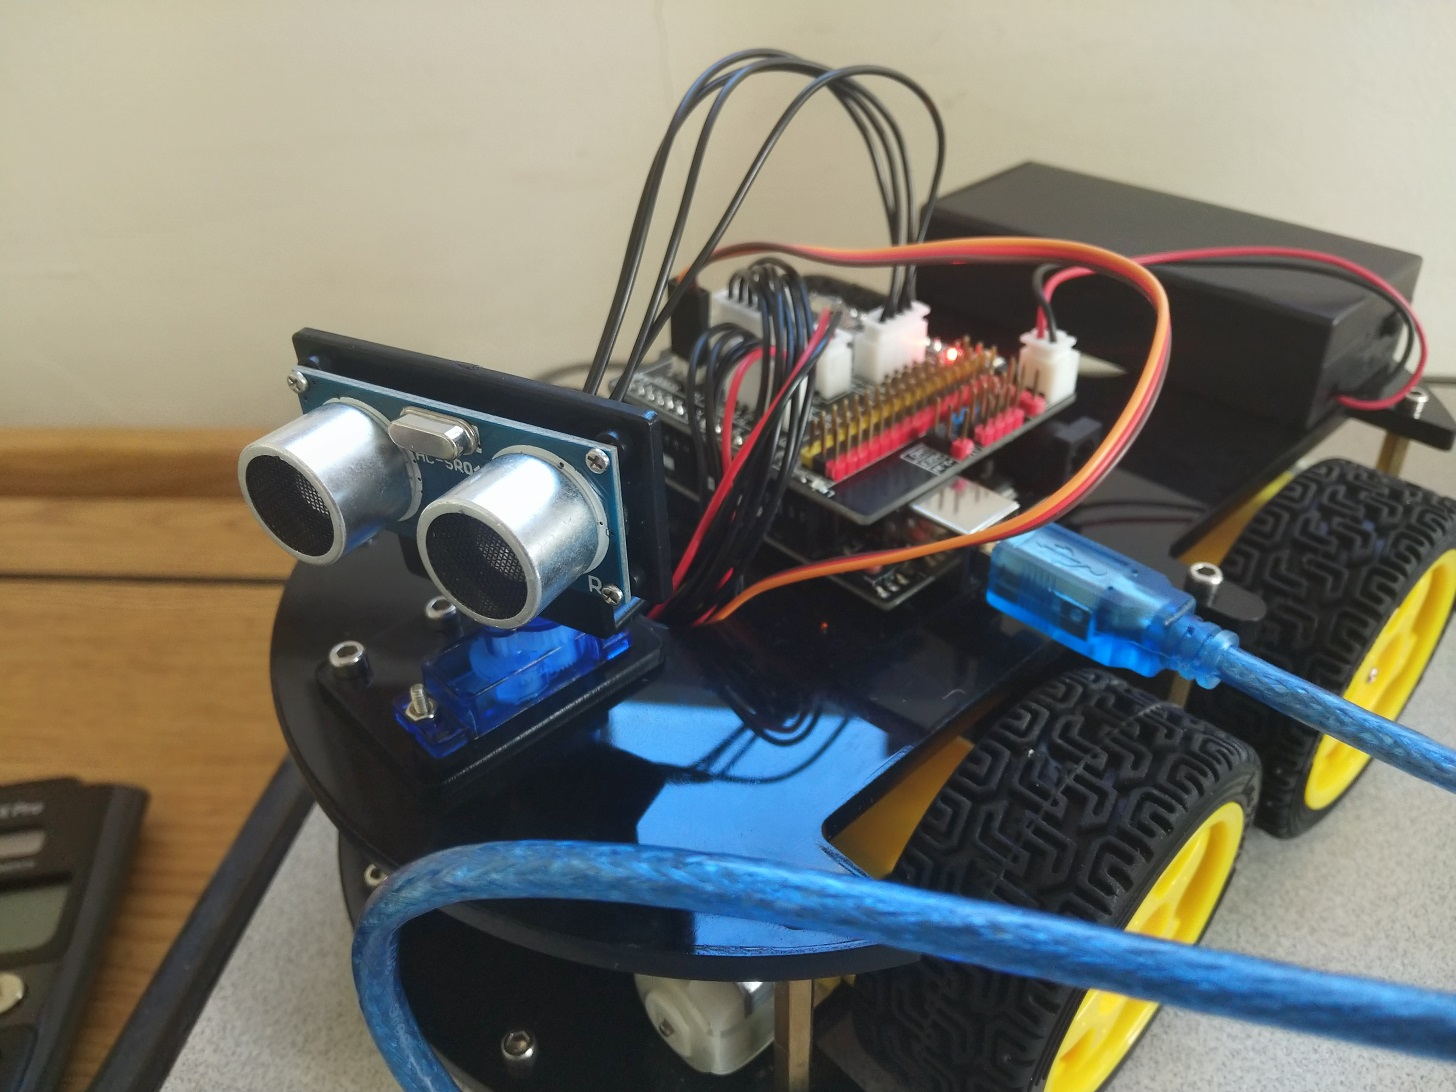
\includegraphics[width=\linewidth]{robot.jpg}
\end{center}
\caption{Robot configuration with ultrasonic sensor.}
\label{fig:f4}
\end{figure}

\section*{Implementation}
For this assignment, we implemented some basic timer control and interfacing logic for the ultrasonic sensor. Additionally, we created the beginning of a pin-change interrupt library to help with controlling the robot later on as the complexity of the assignments increases.\\

In addition to the new code, the motor control code from the last lab assignment has been brought over to the current assignment, and implementation details are reproduced here from the prior assignment.

\subsection*{initPCINT}
Initialization logic for the pin-change interrupts. Sets the pin change interrupt control registers \textit{PCMSK1} and \textit{PCICR} using the defined bit strings \textit{PCMSK1\_CONFIG} and \textit{PCICR\_CONFIG} provided in the file 'pcint.h'.

\subsection*{ISR(PCINT1\_vect) (interrupt)}
Interrupt handler for the second pin change interrupt vector on the board. This assignment only required the use of PCINT12 (PORTC4, pin labeled on the board as A4), which allowed the interrupt to be simplified from the more general approach of capturing the current pin state and comparing with the previous state. This also made the interrupt take less time, and therefore provide a more accurate reading for the distance.

\subsection*{initUltrasonic}
Initialization logic for the ultrasonic sensor and TC1. Configures TC1's overflow interrupt as well as disabling its output pins. starts the timer in the 'off' (disabled) state. TC1 is run in normal mode.

\subsection*{turnoffTimer1}
Helper function to provide a more readable mnemonic for disabling TC1. Works by assigning $0$ to \textit{TCCR1B}.

\subsection*{turnonTimer1}
Helper function to provide a more readable mnemonic for enabling TC1. Works by assigning $0x05$ to \textit{TCCR1B}.

\subsection*{triggerUltrasonic}
Sends a $10\mu{s}$ pulse to the ultrasonic sensor to trigger a 'ping'. Waits $60ms$ after the ping is triggered as suggested in the device's documentation.

\subsection*{getOverflowStatus}
'Getter' function to provide access to the TimerOverflow variable. This can be used to provide specialized behaviors in the event that TC1 overflows while measuring a distance.

\subsection*{receiveUltrasonic}
Reads from TC1 and returns the distance in centimeters corresponding to the time count in TC1. The equation used for this is $(i * 64) / 58$.

\subsection*{TIM16\_ReadTCNT1}
Function to read from TC1 as an atomic operation. Disables the global interrupt bit until the read is completed, stores the timer value into the 'i' local variable, re-enables interrupts, and finally returns 'i'.

\subsection*{TIM16\_WriteTCNT1}
Similar to the read operation, performs an atomic write by disabling the global interrupt bit. the unsigned integer parameter is written into the TCNT1 register, and then interrupts are re-enabled before leaving the function.

\subsection*{initMotor}
All of our motor initializations with timer preparation and 
scaling, PWM modes and timer interrupt enable for turn functions.

\subsection*{setB}
Sets the OCR0B PWM pin and one side of our motor, specifically the 
left side motors on our robot. Set speed and direction with included 
enumeration inside of this motor driver file.

\subsection*{setA}
Sets the OCR0A PWM pin and one side of our motor, specifically the 
right side motors on our robot. Set speed and direction with included 
enumeration inside of this motor driver file.

\subsection*{turnLeft}
Simple abstraction function, activates the proper setB and setA functions 
with speed and length of time to be inside the function then stops.

\subsection*{turnRight}
Simple abstraction function, activates the proper setB and setA functions 
with speed and length of time to be inside the function then stops.

\subsection*{driveForward}
Simple abstraction function, drives the wheels forward for a set amount 
of time, then stops.

\subsection*{driveBackward}
Simple abstraction function, drives the whels backwards for a set amount
of time, then stops.

\subsection*{enum WHEEL\_DIRECTION}
Enumeration to allow ease of programming and simple calls for our motor driver
functions. Values are: 

\begin{itemize}
    \item forward
    \item back
\end{itemize}

\subsection*{ISR(TIMER0\_COMPA\_vect) (interrupt)}
Increments the MAIC by one each time the interrupt is invoked. This allows a rough delay functionality with an accuracy based on the period of the interrupt. The program uses a 1024 prescaler, so the period of a single interrupt cycle is 16ms. We noticed possible errors with this timing method for the smallest prescaler values.

\subsection*{getNumInterruptsForDuration}
Computes the number of PWM periods that need to pass before the specified time has passed, to the next full period. The targetCount global is set to this value and the MAIC (Motor A Interrupt Counter) variable is compared against it to determine when the delay is finished. MAIC is set to 0 at the end of the function to prevent the delay from being incorrect.

\subsection*{delayUntilTargetCount}
After a call to getNumInterruptsForDuration, targetCount will be set and delayUntilTargetCount will spin wait until MAIC is greater than the targetCount. MAIC is incremented by the TIMER0\_COMPA\_vect interrupt so the loop will be escaped after the appropriate delay has gone by.

\subsection*{DELAY\_COUNT}
Macro function to simplify the computation for getNumInterruptsForDuration. Divides the requested speed by the PWM (interrupt) period and adds 1 if the period does not evenly divide the delay.

\section*{Discussion}
The biggest challenge we faced with our approach to this lab was determining what was wrong with our pin change interrupts when they failed to get responses. We found after several experiments and some online research that overly long interrupt handling logic could cause us to miss the rising/falling edges of our sensor. We had written the handler in a general style so it could track the last state and handle changes to multiple pins, but this backfired by taking too much time. The second, and current, version assumed that only one pin would change, allowing us to simplify the logic significantly.\\

This lab provided a useful introduction to using timers and interrupts to provide semi-asynchronous sensor reading and control, which is useful for allowing the robot to move while it is reading in data. Otherwise, we would be required to have the robot stop, take measurements, and then move again.


\section*{Responses}
\begin{enumerate}
\item In this lab we are using timer/counter 1 to generate a dedicated ”clock” for pulse measuring.
The Wiring library provided with the Arduino IDE provides a function pulseIn() which
uses a different timing method. Explain how this pulseIn() function works.

In the native arduino \verb+PulseIn()+ the library is counting the pulse by having calculated the number of clock 
cycles in one spin of a while loop. This property is used to count the status between when the pin changed outputs. 
This of course depends on the number of clock cycles to remain the same in the processor's main frequency, 
and with some software engineering, can be adapted depending on which hardware the compiler is configured for. 
This is in contrast to our method of relying on the Atmega328p's internal timer 1 to count the clock cycles between 
high and low ends of the timer.

\item  Timer/counter 1 is 16 bits, meaning TCNT1 is two bytes wide. With the ATMega328P’s 8-bit
data bus two separate reads must be completed to read TCNT1. In the space of these two
reads, it is possible that TCNT1 changes state. How does the ATMega328P work around this
potential data-integrity hazard?

In the space between these reads the microprocessor has an 8 bit temporary register that handles the 
storage of the high byte while the low byte is being read. The assignment of the high byte then 
happens in the same clock cycle that the data is being written to the temp space.
n the high byte read the arduinio will send the temp register directly to the register to be assigned. This is 
why it is advised to read from the lower register before the higher register when reading two from 16 bit registers.


\end{enumerate} 

\newpage
\section*{Appendices}
Table of contents:
\begin{itemize}
    \item main.c - Handles reading from Ultrasonic sensor and motor control
    \item motor\_driver.h - Motor driver header from lab 5
    \item motor\_driver.c - Motor driver code from lab 5
    \item pcint.h - Pin change interrupt header for ultrasonic sensor
    \item pcint.c - Pin change interrupt code for ultrasonic sensor
    \item pin\_map.h - Pin map header for device
    \item robotio.h - UART control header
    \item robotio.c - UART control code
    \item ultrasonic.h - Ultrasonic header file
    \item ultrasonic.c - Ultrasonic code file
\end{itemize}
\newpage

\section*{Appendix A: main.c}
\begin{tiny}
\lstinputlisting{../main.c}
\end{tiny}
\newpage

\section*{Appendix C: motor\_driver.h}
\begin{tiny}
\lstinputlisting{../motor_driver.h}
\end{tiny}
\newpage

\section*{Appendix D: motor\_driver.c}
\begin{tiny}
\lstinputlisting{../motor_driver.c}
\end{tiny}
\newpage

\section*{Appendix D: pcint.h}
\begin{tiny}
\lstinputlisting{../pcint.h}
\end{tiny}
\newpage

\section*{Appendix E: pcint.c}
\begin{tiny}
\lstinputlisting{../pcint.c}
\end{tiny}
\newpage

\section*{Appendix F: pin\_map.h}
\begin{tiny}
\lstinputlisting{../pin_map.h}
\end{tiny}
\newpage

\section*{Appendix G: robotio.h}
\begin{tiny}
\lstinputlisting{../robotio.h}
\end{tiny}
\newpage

\section*{Appendix H: robotio.c}
\begin{tiny}
\lstinputlisting{../robotio.c}
\end{tiny}
\newpage

\section*{Appendix I: ultasonic.h}
\begin{tiny}
\lstinputlisting{../ultrasonic.h}
\end{tiny}
\newpage

\section*{Appendix J: ultasonic.c}
\begin{tiny}
\lstinputlisting{../ultrasonic.c}
\end{tiny}
\newpage

\end{document}
\grid
